\begin{figure*}[t]
    \centering
    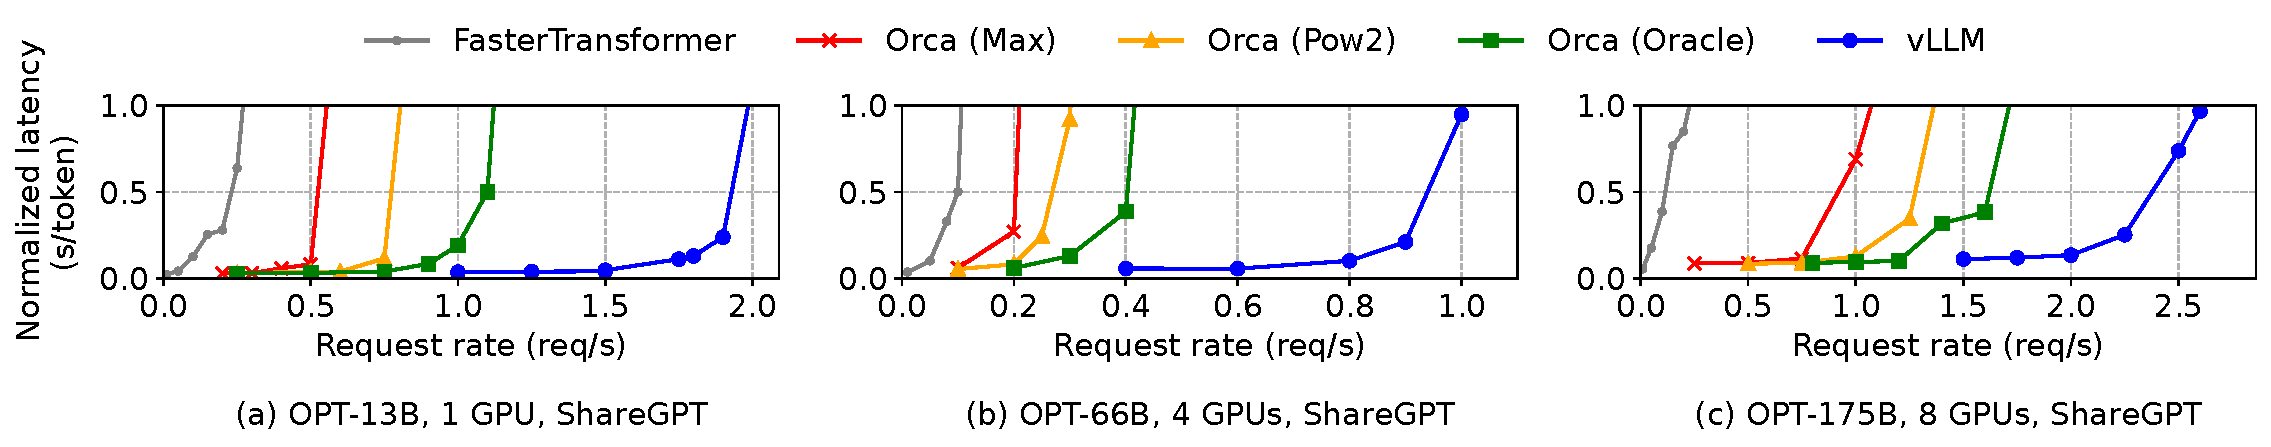
\includegraphics[scale=0.46]{figures/experiments/n1-sharegpt.pdf}
    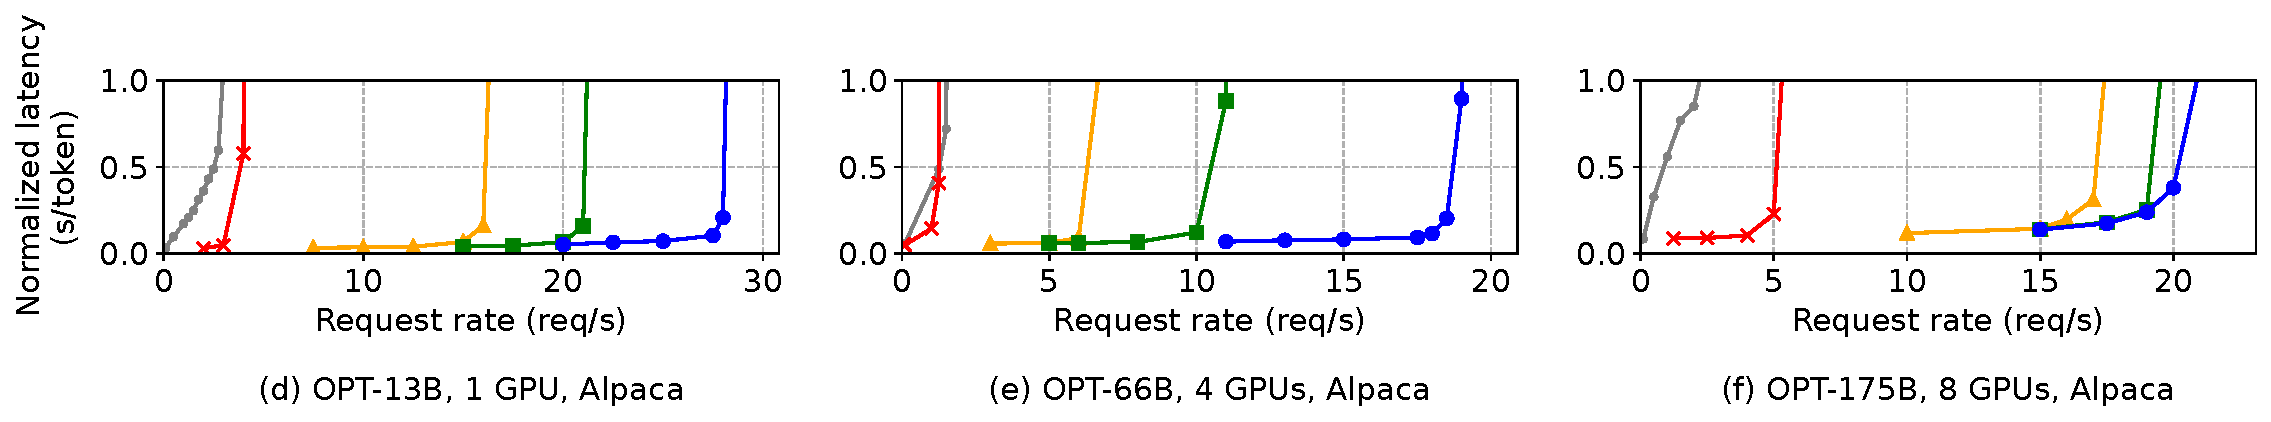
\includegraphics[scale=0.46]{figures/experiments/n1-alpaca.pdf}
\vspace{-8pt}
\caption{Single sequence generation with OPT models on the ShareGPT and Alpaca dataset}
\vspace{-10pt}
\label{fig:single-sequence}
\end{figure*}

\begin{figure}[t]
     \centering
     \begin{subfigure}[t]{0.48\linewidth}
         \centering
         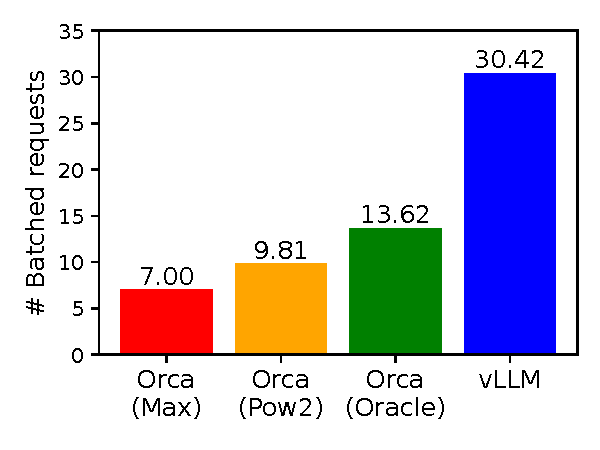
\includegraphics[width=\columnwidth]{figures/experiments/batched_requests_sharegpt.pdf}
         \vspace{-20pt}
         \caption{\small ShareGPT}
     \label{fig:batch-sharegpt}
     \end{subfigure}%\hfill
     \begin{subfigure}[t]{0.48\linewidth}
         \centering
         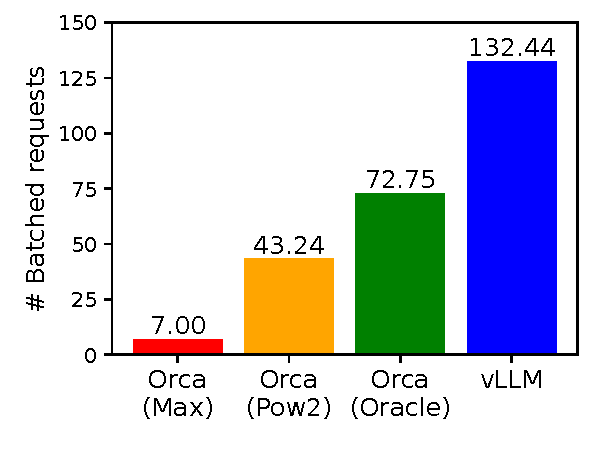
\includegraphics[width=\columnwidth]{figures/experiments/batched_requests_alpaca.pdf}
         \vspace{-20pt}
         \caption{\small Alpaca}
     \label{fig:batch-alpaca}
     \end{subfigure}%\hfill
     \vspace{-8pt}
     \caption{Average number of batched requests when serving OPT-13B for the ShareGPT (2 reqs/s) and Alpaca (30 reqs/s) traces.}
\vspace{-15pt}
\end{figure}

\section{Evaluation}
\label{sec:eval}

In this section, we evaluate the performance of \sys under a variety of workloads.

\subsection{Experimental Setup}
\label{subsec:exp-setup}

\heading{Model and server configurations.}
We use OPT~\cite{zhang2022opt} models with 13B, 66B, and 175B parameters and LLaMA~\cite{touvron2023llama} with 13B parameters for our evaluation.
13B and 66B are popular sizes for LLMs as shown in an LLM leaderboard~\cite{lmsysweek8}, while 175B is the size of the famous GPT-3~\cite{brown2020language} model.
For all of our experiments, we use A2 instances with NVIDIA A100 GPUs on Google Cloud Platform.
The detailed model sizes and server configurations are shown in Table~\ref{table:model_config}.


\heading{Workloads.}
We synthesize workloads based on ShareGPT~\cite{sharegpt} and Alpaca~\cite{alpaca} datasets, which contain input and output texts of real LLM services.
The ShareGPT dataset is a collection of user-shared conversations with ChatGPT~\cite{chatgpt}.
The Alpaca dataset is an instruction dataset generated by GPT-3.5 with self-instruct~\cite{wang2022self}.
We tokenize the datasets and use their input and output lengths to synthesize client requests.
As shown in Fig.~\ref{fig:dataset-length-dist}, the ShareGPT dataset has 8.4$\times$ longer input prompts and 5.8$\times$ longer outputs on average than the Alpaca dataset, with higher variance.
Since these datasets do not include timestamps, we generate request arrival times using Poisson distribution with different request rates.

\heading{Baseline 1: FasterTransformer.}
FasterTransformer~\cite{nvidiaft} is a distributed inference engine highly optimized for latency.
As FasterTransformer does not have its own scheduler, we implement a custom scheduler with a dynamic batching mechanism similar to the existing serving systems such as Triton~\cite{nvidiatriton}.
Specifically, we set a maximum batch size $B$ as large as possible for each experiment, according to the GPU memory capacity.
The scheduler takes up to $B$ number of earliest arrived requests and sends the batch to FasterTransformer for processing.

\begin{figure*}[t]
    \centering
    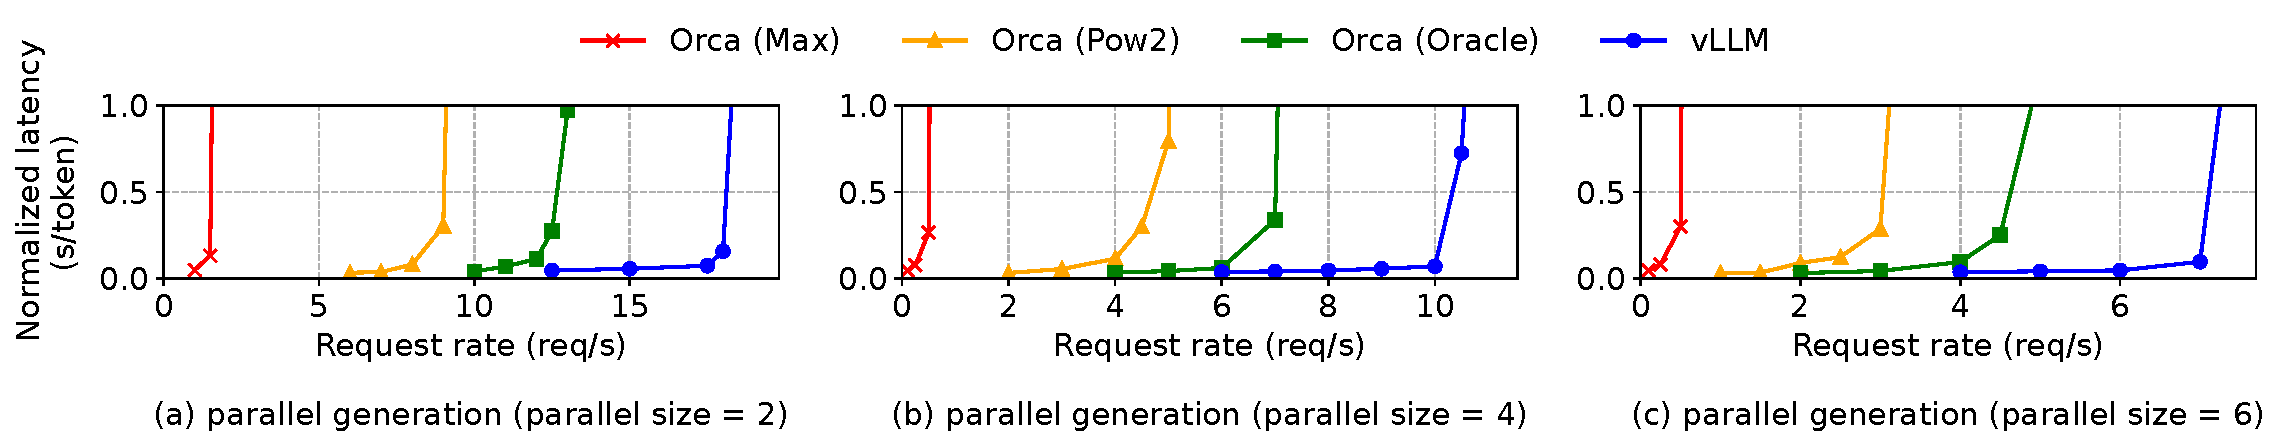
\includegraphics[scale=0.46]{figures/experiments/parallel.pdf}
    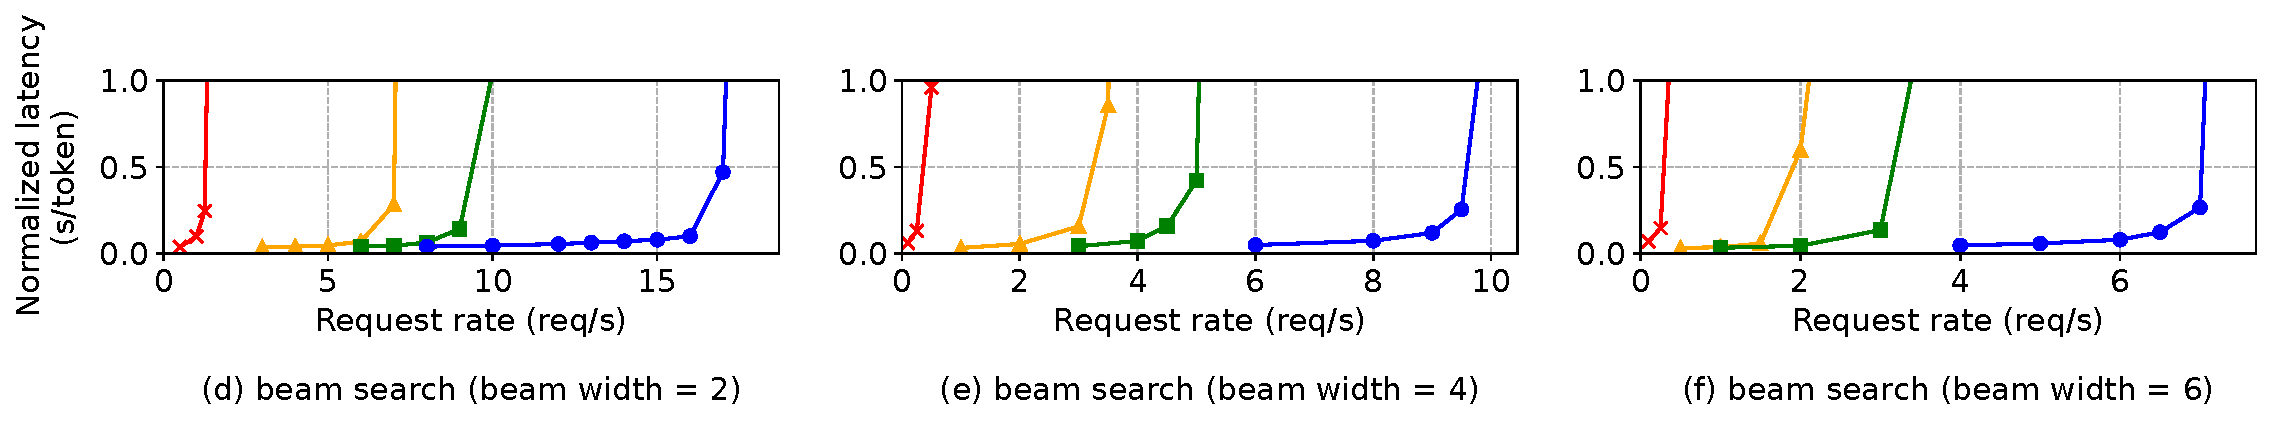
\includegraphics[scale=0.46]{figures/experiments/beam.pdf}
\caption{Parallel generation and beam search with OPT-13B on the Alpaca dataset.}
\label{fig:parallel-beam-alpaca}
\vspace{-5pt}
\end{figure*}


\heading{Baseline 2: Orca.}
Orca~\cite{yu2022orca} is a state-of-the-art LLM serving system optimized for throughput.
Since Orca is not publicly available for use, we implement our own version of Orca.
We assume Orca uses the buddy allocation algorithm to determine the memory address to store KV cache.
We implement three versions of Orca based on how much it over-reserves the space for request outputs:
\begin{CompactItemize}
    \item \textbf{Orca (Oracle).} We assume the system has the knowledge of the lengths of the outputs that will be actually generated for the requests. This shows the upper-bound performance of Orca, which is infeasible to achieve in practice.
    \item \textbf{Orca (Pow2).} We assume the system over-reserves the space for outputs by at most 2$\times$. For example, if the true output length is 25, it reserves 32 positions for outputs.
    \item \textbf{Orca (Max).} We assume the system always reserves the space up to the maximum sequence length of the model, i.e., 2048 tokens.
\end{CompactItemize}

\heading{Key metrics.}
We focus on serving throughput.
Specifically, using the workloads with different request rates, we measure \textit{normalized latency} of the systems, the mean of every request's end-to-end latency divided by its output length, as in Orca \cite{yu2022orca}.
A high-throughput serving system should retain low normalized latency against high request rates.
For most experiments, we evaluate the systems with 1-hour traces.
As an exception, we use 15-minute traces for the OPT-175B model due to the cost limit.

\subsection{Basic Sampling}
\label{sec:eval:basic-sampling}

We evaluate the performance of \sys with basic sampling (one sample per request) on three models and two datasets.
The first row of Fig.~\ref{fig:single-sequence} shows the results on the ShareGPT dataset.
The curves illustrate that as the request rate increases, the latency initially increases at a gradual pace but then suddenly explodes.
This can be attributed to the fact that when the request rate surpasses the capacity of the serving system, the queue length continues to grow infinitely and so does the latency of the requests.

On the ShareGPT dataset, \sys can sustain $1.7\times$--$2.7\times$ higher request rates compared to Orca (Oracle) and $2.7\times$--$8\times$ compared to Orca (Max), while maintaining similar latencies.
This is because \sys's \tech can efficiently manage the memory usage and thus enable batching more requests than Orca.
For example, as shown in Fig.~\ref{fig:batch-sharegpt}, for OPT-13B vLLM processes $2.2\times$ more requests at the same time than Orca (Oracle) and $4.3\times$ more requests than Orca (Max).
Compared to FasterTransformer, \sys can sustain up to $22\times$ higher request rates, as FasterTransformer does not utilize a fine-grained scheduling mechanism and inefficiently manages the memory like Orca (Max).

The second row of Fig.~\ref{fig:single-sequence} and Fig.~\ref{fig:batch-alpaca} shows the results on the Alpaca dataset, which follows a similar trend to the ShareGPT dataset.
One exception is Fig.~\ref{fig:single-sequence} (f), where \sys's advantage over Orca (Oracle) and Orca (Pow2) is less pronounced.
This is because the model and server configuration for OPT-175B (Table~\ref{table:model_config}) allows for large GPU memory space available to store KV cache, while the Alpaca dataset has short sequences.
In this setup, Orca (Oracle) and Orca (Pow2) can also batch a large number of requests despite the inefficiencies in their memory management.
As a result, the performance of the systems becomes compute-bound rather than memory-bound.


\begin{figure}[t]
     \centering
     \begin{subfigure}[b]{0.5\linewidth}
         \centering
         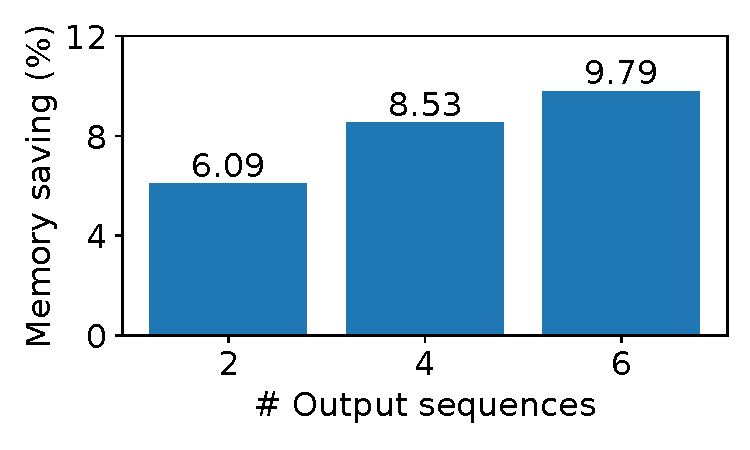
\includegraphics[width=.9\columnwidth]{figures/experiments/mem_saving_parallel_gen.pdf}
         \vspace{-5pt}
         \caption{Parallel sampling}
     \end{subfigure}%\hfill
     \begin{subfigure}[b]{0.5\linewidth}
         \centering
         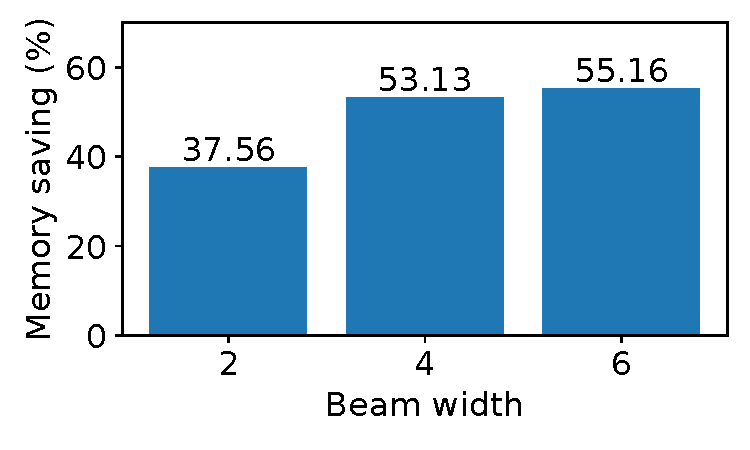
\includegraphics[width=.9\columnwidth]{figures/experiments/mem_saving_beam.pdf}
         \vspace{-5pt}
         \caption{Beam search}
     \end{subfigure}%\hfill
     \vspace{-7pt}
     \caption{Average amount of memory saving from sharing KV blocks, when serving OPT-13B for the Alpaca trace.}
    \vspace{-12pt}
\label{fig:memory-saving-sharing}
\end{figure}


\subsection{Parallel Sampling and Beam Search}
\label{sec:eval:beamsearch}

We evaluate the effectiveness of memory sharing in \tech with two popular sampling methods: parallel sampling and beam search.
In parallel sampling, all parallel sequences in a request can share the KV cache for the prompt.
As shown in the first row of Fig.~\ref{fig:parallel-beam-alpaca}, with a larger number of sequences to sample, \sys brings more improvement over the Orca baselines.
Similarly, the second row of Fig.~\ref{fig:parallel-beam-alpaca} shows the results for beam search with different beam widths.
Since beam search allows for more sharing, \sys demonstrates even greater performance benefits.
The improvement of \sys over Orca (Oracle) on OPT-13B and the Alpaca dataset goes from $1.3 \times$ in basic sampling to $2.3 \times$ in beam search with a width of 6.

Fig.~\ref{fig:memory-saving-sharing} plots the amount of memory saving, computed by the number of blocks we saved by sharing divided by the number of total blocks without sharing. We show 6.1\% - 9.8\% memory saving on parallel sampling and 37.6\% - 55.2\% on beam search.
In the same experiments with the ShareGPT dataset, we saw 16.2\% - 30.5\% memory saving on parallel sampling and 44.3\% - 66.3\% on beam search.



\subsection{Shared prefix}

We explore the effectiveness of \sys for the case a prefix is shared among different input prompts, as illustrated in Fig.~\ref{fig:share-prompt}.
For the model, we use LLaMA-13B~\cite{touvron2023llama}, which is multilingual.
For the workload, we use the WMT16~\cite{bojar-EtAl:2016:WMT1} English-to-German translation dataset and synthesize two prefixes that include an instruction and a few translation examples.
The first prefix includes a single example (i.e., one-shot) while the other prefix includes 5 examples (i.e., few-shot).
As shown in Fig.~\ref{fig:prefix-share-exp} (a), \sys achieves $1.67 \times$ higher throughput than Orca (Oracle) when the one-shot prefix is shared.
Furthermore, when more examples are shared (Fig.~\ref{fig:prefix-share-exp} (b)), \sys achieves $3.58 \times$ higher throughput than Orca (Oracle).

\begin{figure}[t]
    \centering
    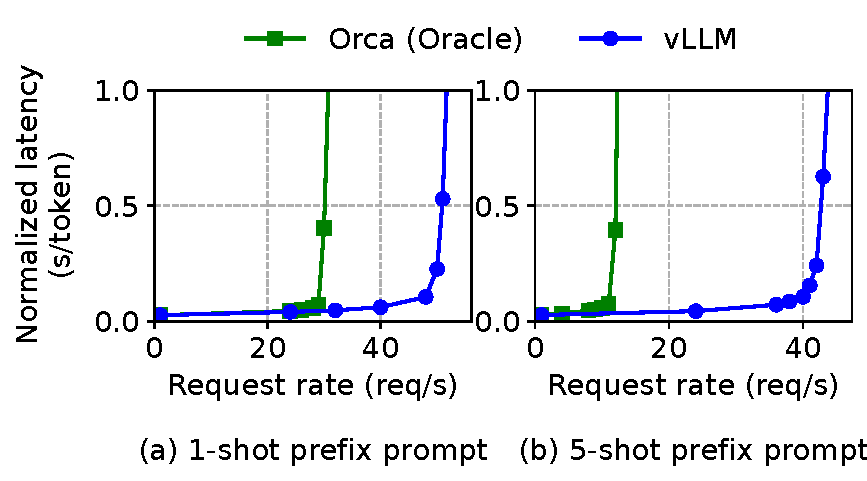
\includegraphics[width=.9\columnwidth]{figures/experiments/prefix.pdf}
    \vspace{-5pt}
    \caption{Translation workload where the input prompts share a common prefix. The prefix includes (a) 1 example with 80 tokens or (b) 5 examples with 341 tokens.}
\label{fig:prefix-share-exp}
\end{figure}

\begin{figure}
    \centering
    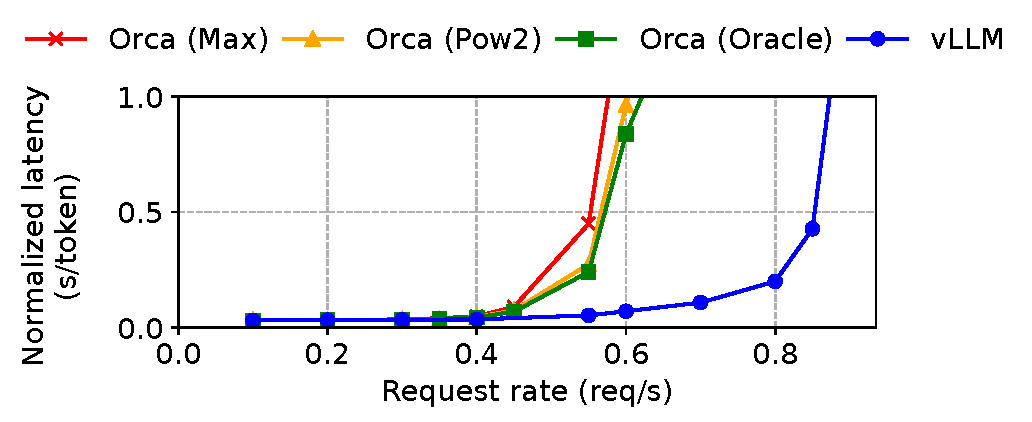
\includegraphics[width=0.8\columnwidth]{figures/experiments/chat-sharegpt.pdf}
    \vspace{-7pt}
    \caption{Performance on chatbot workload.}
    \label{fig:chatbot}
\end{figure}

\subsection{Chatbot}
\label{sec:chatbot}
A chatbot \cite{chatgpt, bard, vicuna2023} is one of the most important applications of LLMs.
To implement a chatbot, we let the model generate a response by concatenating the chatting history and the last user query into a prompt.
We synthesize the chatting history and user query using the ShareGPT dataset.
Due to the limited context length of the OPT-13B model, we cut the prompt to the last 1024 tokens and let the model generate at most 1024 tokens.
We do not store the KV cache between different conversation rounds as doing this would occupy the space for other requests between the conversation rounds.

Fig.~\ref{fig:chatbot} shows that \sys can sustain $2\times$ higher request rates compared to the three Orca baselines.
Since the ShareGPT dataset contains many long conversations, the input prompts for most requests have 1024 tokens.
Due to the buddy allocation algorithm, the Orca baselines reserve the space for 1024 tokens for the request outputs, regardless of how they predict the output lengths.
For this reason, the three Orca baselines behave similarly.
In contrast, \sys can effectively handle the long prompts, as \tech resolves the problem of memory fragmentation and reservation.
